\renewcommand{\thislecture}{7 }

%
% Cover page
%

\title[Neutrino Physics / Lecture \thislecture]
{
  {\huge \color{yellow} Neutrino Physics - Lecture \thislecture} \\
  {\it Quasi-Elastic Neutrino Scattering}\\
}

\author[C.Andreopoulos] {
  Professor Costas Andreopoulos\inst{1,2}
}
\institute[Liverpool/STFC-RAL] {
   \inst{1} University of Liverpool,
   \inst{2} STFC Rutherford Appleton Laboratory\\
   \vspace{0.5cm}
   {\it {\color{magenta} A post-graduate student lecture course}}\\
   \vspace{0.2cm}
}
\date{\today}

\titlegraphic{
  
\includegraphics[height=25px]{./images/logo/liverpool.png}
  \hspace{3px}
  
\includegraphics[height=30px]{./images/logo/ral.png}
}

	



\begin{frame}[plain]
  \titlepage
\end{frame}

%
% Outline
%

\begin{frame}{Outline for Lecture \thislecture}


\end{frame}


%
% Quasi-elastic scattering / Generalities
%

\begin{frame}{Charged Current Quasi-elastic (CCQE) scattering}
\begin{columns}
  \begin{column}{0.50\textwidth}
   \begin{center}
    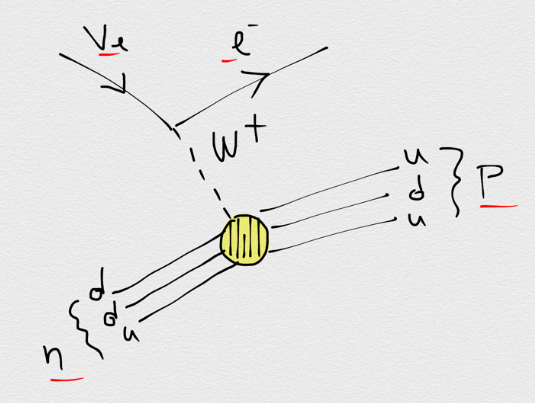
\includegraphics[width=0.90\textwidth]{./images/nuint/feyn/ccqe_feynman_diagram_0.png}\\
    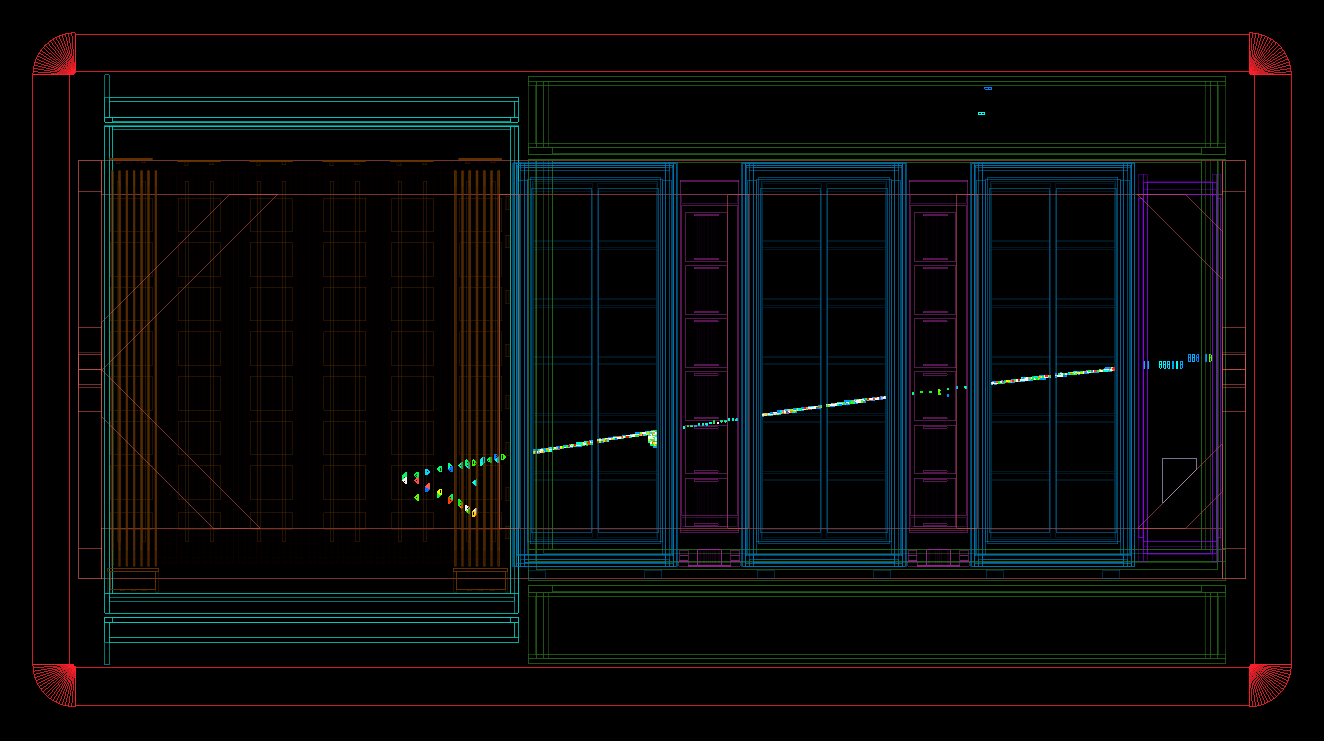
\includegraphics[width=0.90\textwidth]{./images/nuint/evdisplay/ccqe_t2k_p0d_event_display_0.png}\\
    {\tiny Event display from http://homepages.warwick.ac.uk/$\sim$phrfba/}
    \end{center}
  \end{column}
  \begin{column}{0.50\textwidth}
    $\nu_{l} + n \rightarrow l^{-} + p$\\
    $\bar{\nu}_{l} + p \rightarrow l^{+} + n$\\
    \begin{itemize}
    {\scriptsize
     \item Dominant process at $\sim$ 1 GeV
     \item Simple topology
      The neutrino scatters elastically off the nucleon (does not excite or break it up).\\
      Easy identification and reconstruction
     \item Simple energy reconstruction owing to quasi two body kinematics
     \item Golden channel for oscillation studies at $\sim$ 1 GeV
    }
    \end{itemize}
  \end{column}
\end{columns}
\end{frame}


\begin{frame}{Neutrino energy reconstruction in CCQE scattering}

\begin{equation*}
   E_{\nu}^{reco} = \frac{m_p^2 - (m_N-E_b)^2 - m_l^2 + 2(m_N-E_b)E_l}
                         {2(m_N-E_b-E_{\mu}+|{\bf p_l}|cos\theta_l)}
\end{equation*}

\begin{equation*}
   Q^2_{reco} = 2  E_{\nu;reco} (E_l - |{\bf p_l}|cos\theta_l) - m_l^2
\end{equation*}

 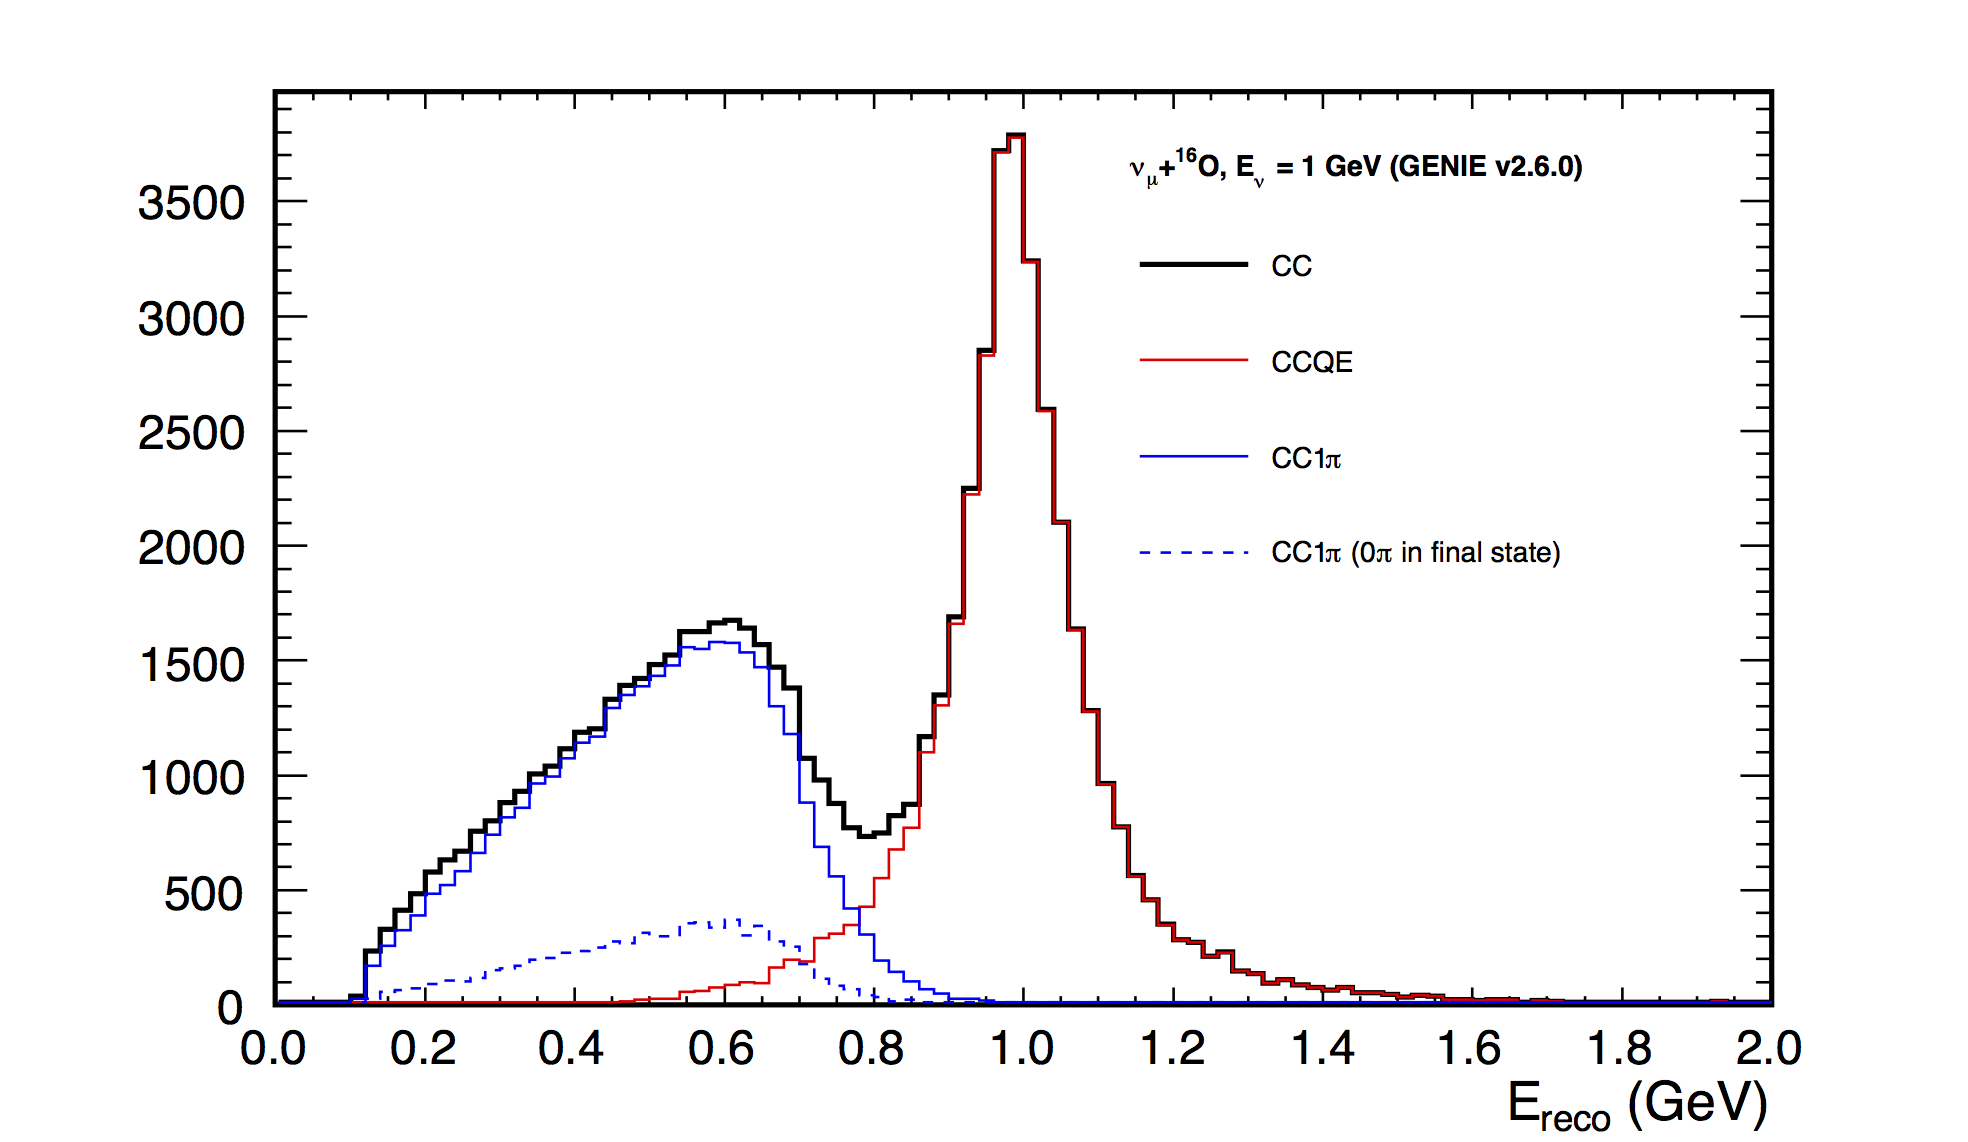
\includegraphics[width=0.90\textwidth]{./images/nuint/ccqe/ereco_numuO16_1GeV.png}\\

\end{frame}


%
%
%

\begin{frame}{ep}

\begin{equation*}
  M = \frac{e^2}{q^2} \Big( \bar{u}_{e}(k^{\prime}) \gamma^{\mu} u_{e}(k) \Big) J_{\mu}
\end{equation*}


Two form factors needed to describe elastic scattering of electrons by spin $\frac{1}{2}$ nucleons:
\begin{itemize}
 \item one form factor (Dirac form factor, $F_1$) for the case where the spin state of the nucleon is the same in the initial and final states, and
 \item one form factor (Pauli form factor, $F_2$) for the case where the spin flips.
\end{itemize}

\begin{equation*}
   J^{\mu}(q^2) \propto \bar{u}_{N}(p^{\prime}) \Big[
       {\color{magenta}F_{1}(q^2)}\gamma^{\mu} +
       \frac{1}{2m_{N}} {\color{magenta}F_{2}(q^2)}{\sigma}^{\mu\nu} p_{\nu}
      \Big] u_{N}(p)
\end{equation*}


\begin{equation*}
  F_{1}^{(p)} = 1,\;\;
  F_{2}^{(p)} = \kappa_{p},\;\;
  F_{1}^{(n)} = 1\;\;
  F_{2}^{(n)} = \kappa_{n}
\end{equation*}

where $\kappa_{p}$ = $\mu_{p}$-1 and $\kappa_{n}$ = $\mu_{n}$ are the anomalous magnetic moments of the proton and neutron respectively,
$\mu_{p}$ (=2.7928$\mu_{N}$) and $\mu_{n}$ (=-1.9130$\mu_{N}$)are the magnetic moments of the proton and neutron respectively,
and $\mu_{N}$ is the nuclear magneton.

\end{frame}

%
%
%

\begin{frame}{ep}

Experimentalists typically use two linear combinations of $F_{1}$ and $F_{2}$ vector form factors:
The electric form factor $G_{E}$ and the magnetic form factor $G_{M}$:

\begin{equation*}
  G_{E} = F_{1} - \tau F_{2} \;\; and \;\; G_{M} = F_{1} + F_{2}
\end{equation*}

where $\tau = Q^{2}/4m_{N}^{2}$

For low momentum transfers, $G_{E}$ and $G_{M}$ are the Fourier transforms of the
nucleon charge and magnetization current densities.

\end{frame}

%
%
%

\begin{frame}{ep}

\begin{equation*}
  \frac{d\sigma}{d\Omega} =
     \sigma_{M} \frac{E^{\prime}}{E}
     \Big( \frac{ G^{2}_{E}(Q^2) + \tau G^{2}_{M}(Q^2) }{ 1+\tau } +
           2 \tau G^{2}_{M}(Q^2) tan^{2}\frac{\theta}{2} \Big)
\end{equation*}

where
$\sigma_{M}$ is the Mott cross-section

\end{frame}


%
%
%

\begin{frame}{Nucleon form factor measurements}

\begin{itemize}
  \item Rosenbluth separation measurements
  \item Polarization measurements
\end{itemize}

\end{frame}

%
%
%

\begin{frame}{Rosenbluth separation}

\begin{columns}
  \begin{column}{0.50\textwidth}

    \begin{equation*}
      \frac{d\sigma}{d\Omega} =
        \frac { \alpha^2 E'_{e} cos^{2}\frac{\theta}{2} }
              { 4 E_{e}^{3} sin^{4}\frac{\theta}{2} }
        \cdot
        \Big(
          G_{e}^{2}(Q^2) + \frac{\tau}{\epsilon} G_{e}^{2}(Q^2)
        \Big)
        \cdot
        \Big(
          \frac{1}{1+\tau}
        \Big)
    \end{equation*}

  \end{column}
  \begin{column}{0.50\textwidth}
   \begin{center}
    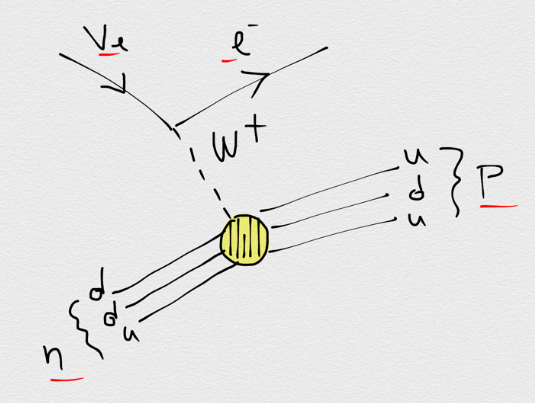
\includegraphics[width=0.90\textwidth]{./images/nuint/feyn/ccqe_feynman_diagram_0.png}\\
   \end{center}
  \end{column}
\end{columns}

\end{frame}

%
%
%

\begin{frame}{Blah}

\begin{equation*}
  \frac{G_{e}}{G_{m}} =
      - \frac{P_{T}}{P_{L}}
      \cdot
      \frac{E_{e}+E_{e}'}{2M}
      \cdot
      tan\Big( \frac{\theta}{2} \Big)
\end{equation*}

\end{frame}

%
%
%

\begin{frame}{From electron to neutrino scattering}

The formalism is similar.

But for neutrino scattering, the {\em axial current} of nucleon has to be included in addition.

\begin{equation*}
   J^{\mu}_{A}(Q^2) = \bar{u}_{N}(p^{\prime}) \Big[
       G_{A}(Q^2) \gamma^{\mu} +
       \frac{1}{2m_{N}} G_{P}(Q^2) q^{\mu}
      \Big] \gamma^{5} u_{N}(p)
\end{equation*}

where $G_{P}$ is a pseudoscalar form factor determined by PCAC
\begin{equation*}
 G_{P}(Q^2) = \frac{4m_{N}^{2} G_A(Q^2)}{m_{\pi}^{2}+Q^{2}}
\end{equation*}

\end{frame}


%
%
%

\begin{frame}{CCQE cross-section}

Lorentz symmetry allows us to write the differential CCQE cross-section as:\\

\begin{equation*}
  \frac{d\sigma}{dQ^2} =
     \frac{G_F^2 |V_{ud}|^2 M^2}{8 \pi E_{\nu}^2}
     \Big(
       {\color{magenta} A(Q^2) } \mp
       {\color{magenta} B(Q^2) } \cdot \frac{s-u}{M^2} +
       {\color{magenta} C(Q^2) } \cdot (\frac{s-u}{M^2})^2
     \Big)
\end{equation*}

where
\begin{itemize}
 \item $G_{F}$
 \item $V_{ud}$
 \item $M$
 \item s,u
 \item $E_{\nu}$
 \item $Q^{2}$
\end{itemize}

\end{frame}


%
%
%

\begin{frame}{CCQE cross-section}

Lorentz symmetry allows us to write the differential CCQE cross-section as:\\

\begin{equation*}
  \frac{d\sigma}{dQ^2} =
     \frac{G_F^2 |V_{ud}|^2 M^2}{8 \pi E_{\nu}^2}
     \Big(
       {\color{magenta} A(Q^2) } \mp
       {\color{magenta} B(Q^2) } \cdot \frac{s-u}{M^2} +
       {\color{magenta} C(Q^2) } \cdot (\frac{s-u}{M^2})^2
     \Big)
\end{equation*}

$A(Q^2)$, $B(Q^2)$ and $C(Q^2)$ functions of the
\begin{itemize}
  \item $F_{v}^{1}$, $F_{v}^{2}$ vector form factors
  \begin{itemize}
    \item determined from electron scattering via CVC
  \end{itemize}
  \item $F_{A}$ axial vector form factor
  \begin{itemize}
    \item dipole form is  usually assumed\\
      \begin{equation*}
         F_{A}(Q^2) = g_{A} (1 + \frac{Q^2}{M_A^{2}})^{-2}
      \end{equation*}
  \end{itemize}
\end{itemize}

\end{frame}

%
%
%

\begin{frame}{CCQE cross-section}

\begin{equation*}
 A = \frac{m^2+Q^2}{M^2}
     \Big(
       (1+\tau) G_A^2 - (1-\tau) F_1^2 + \tau(1-\tau) F_2^2 + 4 \tau F_1 F_2 -
       \frac{m^2}{4M^2} ...
     \Big)
\end{equation*}

\begin{equation*}
 B = \frac{Q^2}{M^2} G_A (F_1 + F_2)
\end{equation*}

\begin{equation*}
 C = \frac{1}{4} (G_A^2 + F_1^2 + F_2^2)
\end{equation*}

\end{frame}


%
% Vector form factors
%

\begin{frame}{Vector form factors}

Vectors form factors $F_{v}^{1}$, $F_{v}^{2}$ can be expressed in terms of the electric and
magnetic nucleon form factors $G_{E}(Q^2)$ and $G_{M}(Q^{2})$

\begin{equation*}
     F_{v}^{1}(Q^2) = \frac {G_{E}(Q^2) - \tau G_{M}(Q^2)} {1-\tau}
 \xi F_{v}^{2}(Q^2) = \frac {G_{M}(Q^2) -      G_{E}(Q^2)} {1-\tau}
\end{equation*}

CVC allows the determination of $G_{E}(Q^2)$ and $G_{M}(Q^{2})$ from the elastic nucleon form factors

\begin{equation*}
   G_{E}(Q^2) =  G_{ep}(Q^2) -  G_{en}(Q^2)
   G_{M}(Q^2) =  G_{mp}(Q^2) -  G_{mn}(Q^2)
\end{equation*}

\end{frame}

%
% Neutrino CCQE measurements
%

\begin{frame}{Neutrino CCQE measurements}

\begin{itemize}
\item 1
\item 2
\item 3
\end{itemize}

\end{frame}


%
% Bubble chambers
%

\begin{frame}{Bubble chamber CCQE measurements}

\begin{columns}
  \begin{column}{0.33\textwidth}
   \begin{center}
     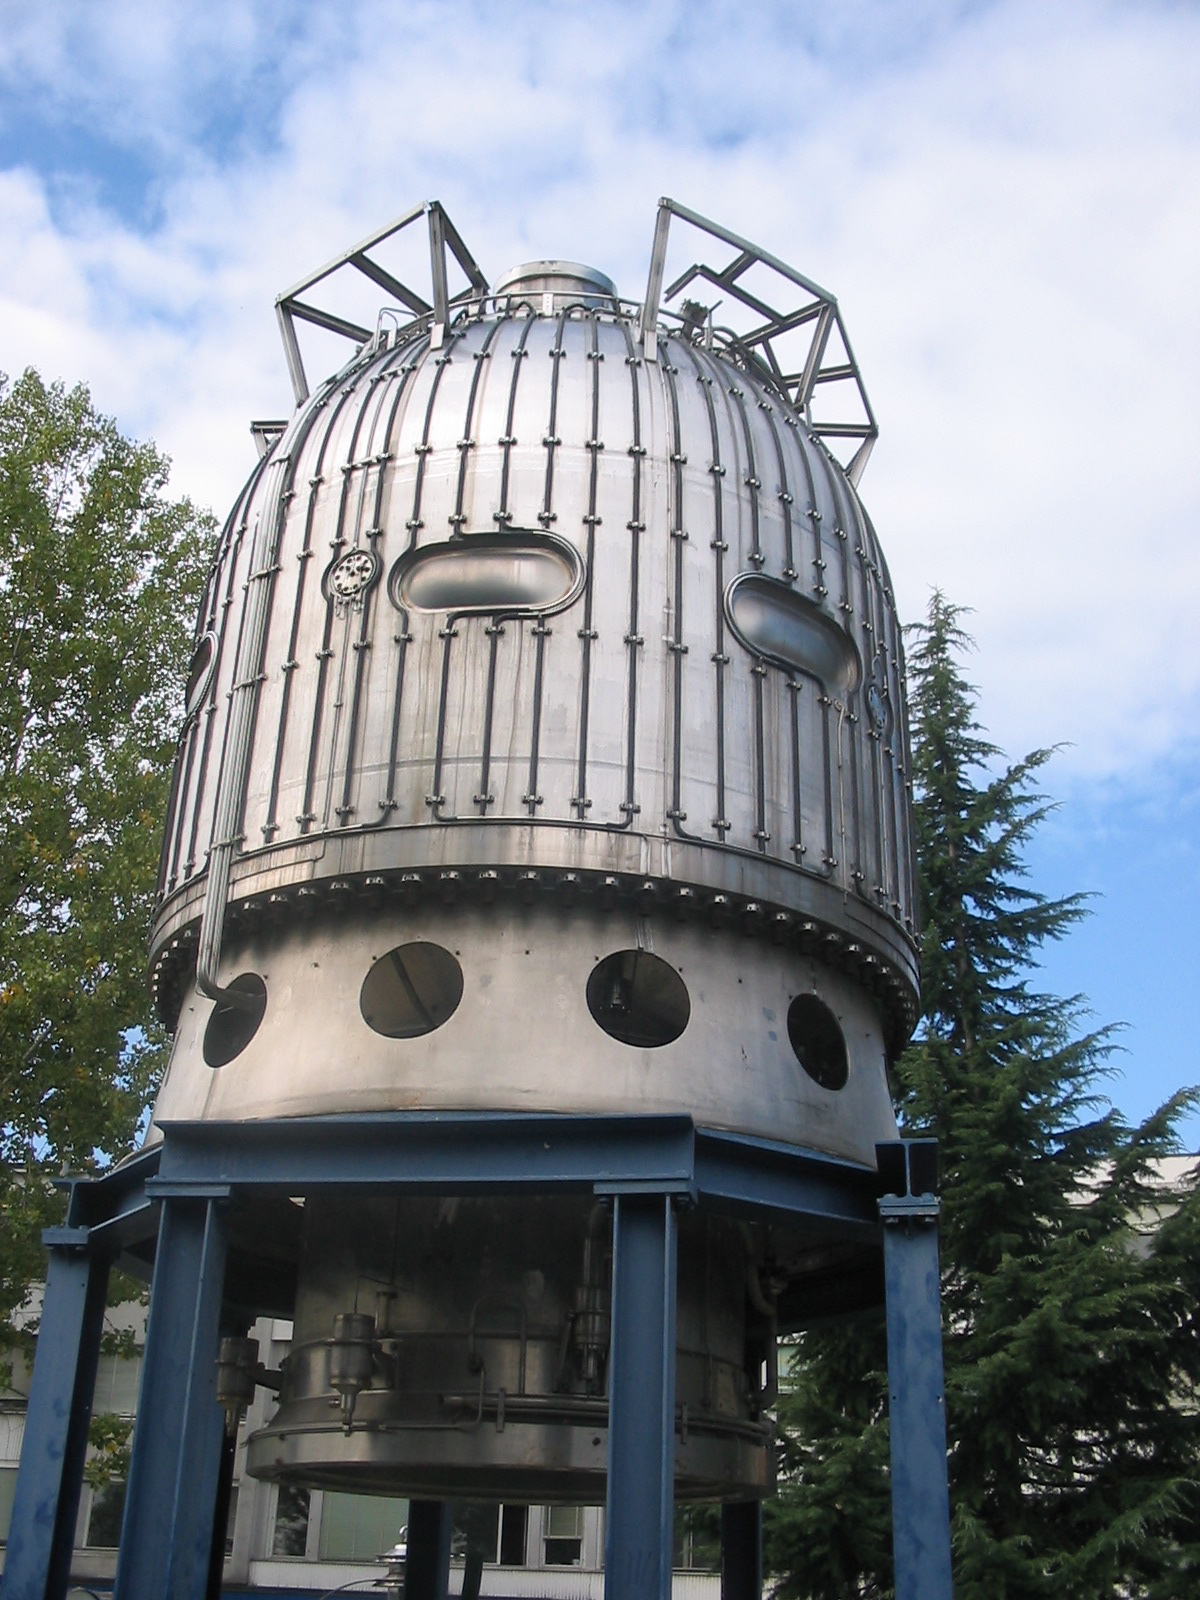
\includegraphics[width=0.90\textwidth]{./images/bc/bebc.jpg}\\
     {\small BEBC}
    \end{center}
  \end{column}
  \begin{column}{0.33\textwidth}
   \begin{center}
     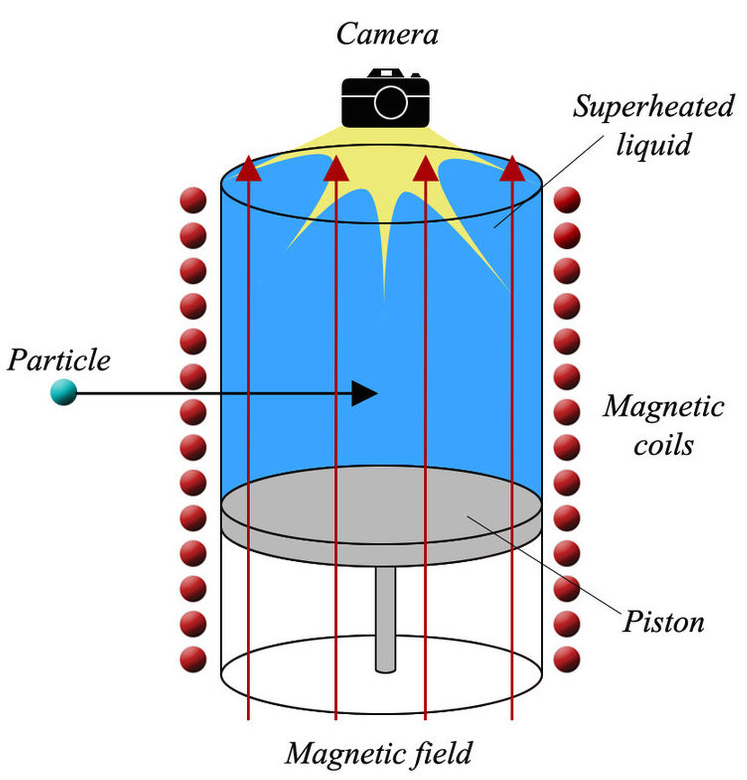
\includegraphics[width=0.98\textwidth]{./images/bc/principle_of_operation.png}\\
    \end{center}
  \end{column}
  \begin{column}{0.33\textwidth}
   \begin{center}
     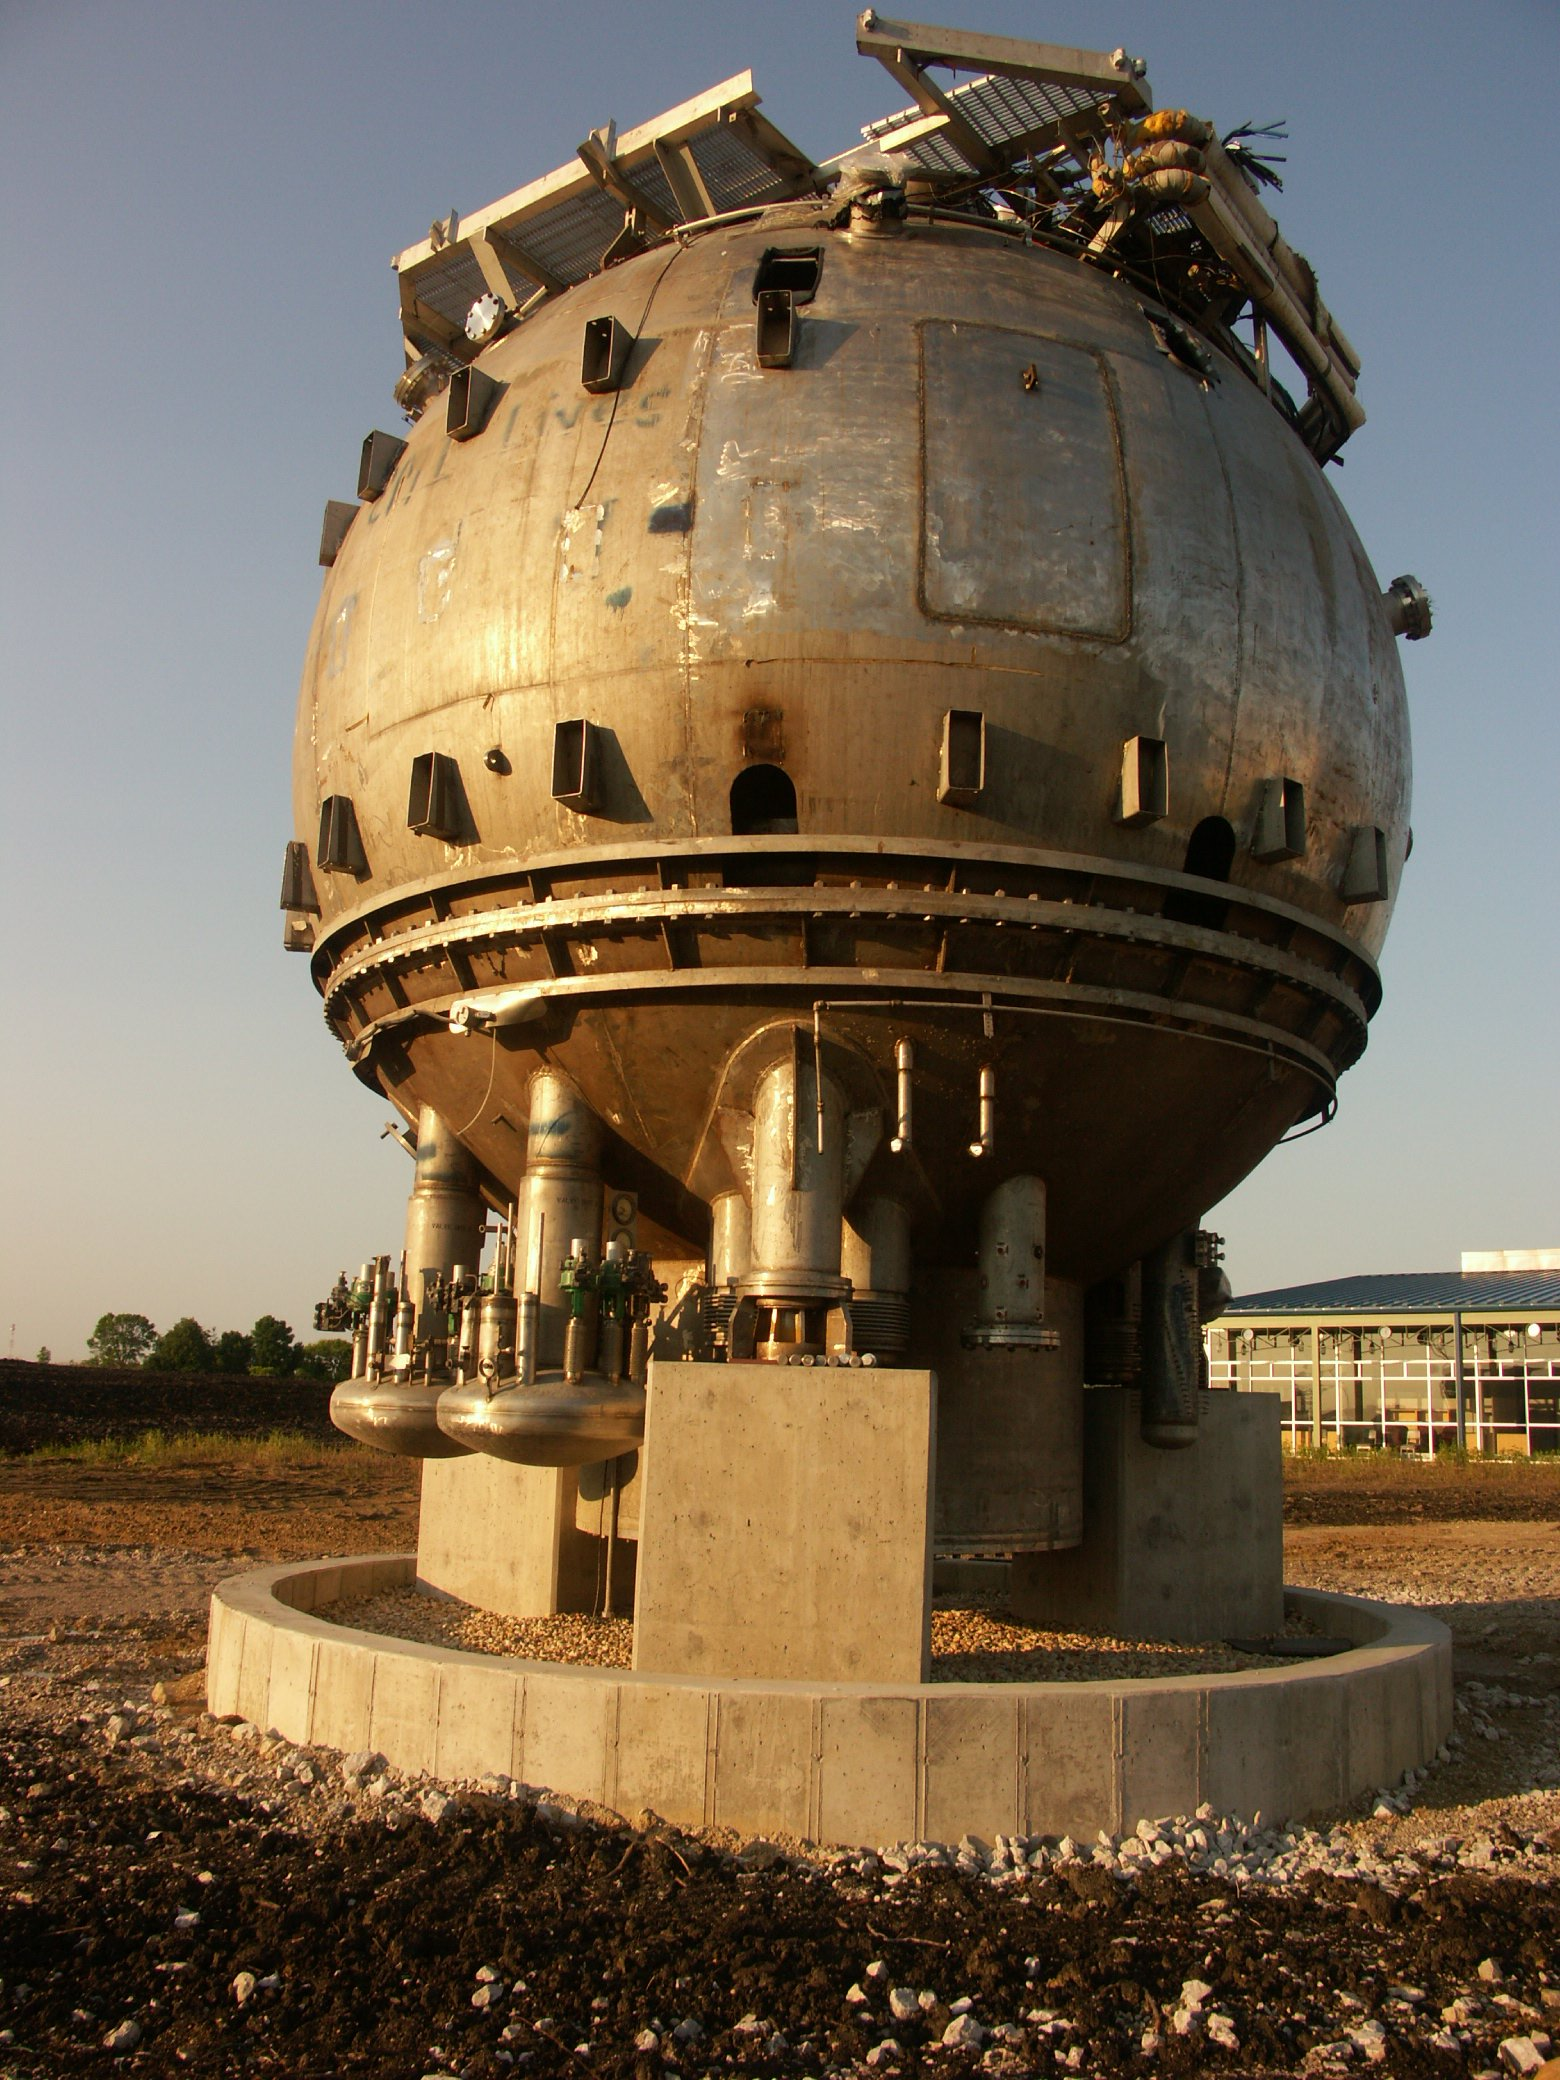
\includegraphics[width=0.90\textwidth]{./images/bc/fnal_15ft.jpg}\\
     {\small FNAL-15ft}
    \end{center}
  \end{column}
\end{columns}

\end{frame}


%
%
%

\begin{frame}{Bubble chamber CCQE measurements}

\begin{center}
  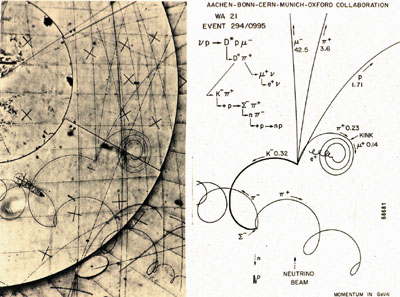
\includegraphics[width=0.80\textwidth]{./images/bc/nu_event_display_and_schematic_1.jpg}\\
\end{center}

\end{frame}


%
% Bubble chambers
%

\begin{frame}{Bubble chamber CCQE measurements}

\begin{center}
 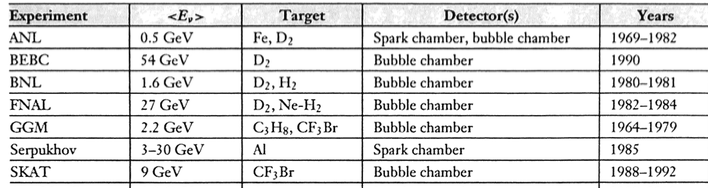
\includegraphics[width=0.75\textwidth]{./images/nuint/ccqe/pre1990_investigations_1.png}\\
 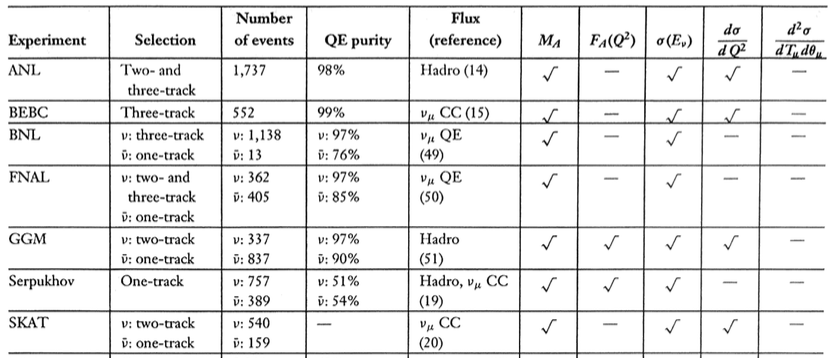
\includegraphics[width=0.83\textwidth]{./images/nuint/ccqe/pre1990_investigations_2.png}\\
 {\scriptsize \color{blue}[Gallagher, Garvey, Zeller, Annu.Rev.Nucl.Part.Sci. 2011, 61:355-78]}\\
\end{center}
\end{frame}

%
% Bubble chambers
%

\begin{frame}{Bubble chamber CCQE measurements}

CCQE measurements primarily in deuterium targets

$\nu_{l} + d \rightarrow l^{-} + p + p$

Both nucleons can be identified / reconstructed
High purity and efficiency
No significant nuclear effects

\end{frame}

%
%
%

\begin{frame}{K2K and early MiniBooNE CCQE measurements}

\end{frame}

%
%
%

\begin{frame}{MiniBooNE CCQE measurements}

\end{frame}

%
%
%

\begin{frame}{SciBooNE CCQE measurements}

\end{frame}

%
%
%

\begin{frame}{NOMAD CCQE measurements}

\end{frame}

%
%
%

\begin{frame}{T2K CCQE measurements}

\end{frame}

%
%
%

\begin{frame}{MINOS CCQE measurements}

\end{frame}


%
%
%
\begin{frame}{The QE puzzle}

\begin{itemize}
  {\small
  \item QE: A {\bf golden channel} for oscillation searches at T2K/HK.\\
  \item 2-body kinematics: $E_{\nu}$ reconstruction from lepton momentum/angle.\\
  }
\end{itemize}

  \begin{columns}
    \begin{column}{0.42\textwidth}
      \begin{center}
         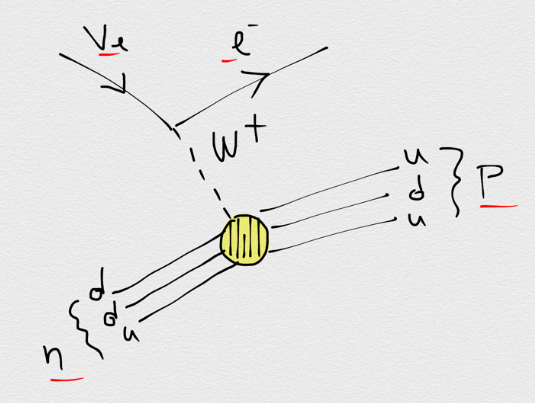
\includegraphics[width=0.82\textwidth]{./images/nuint/feyn/ccqe_feynman_diagram_0}\\
         \vspace{0.2cm}
         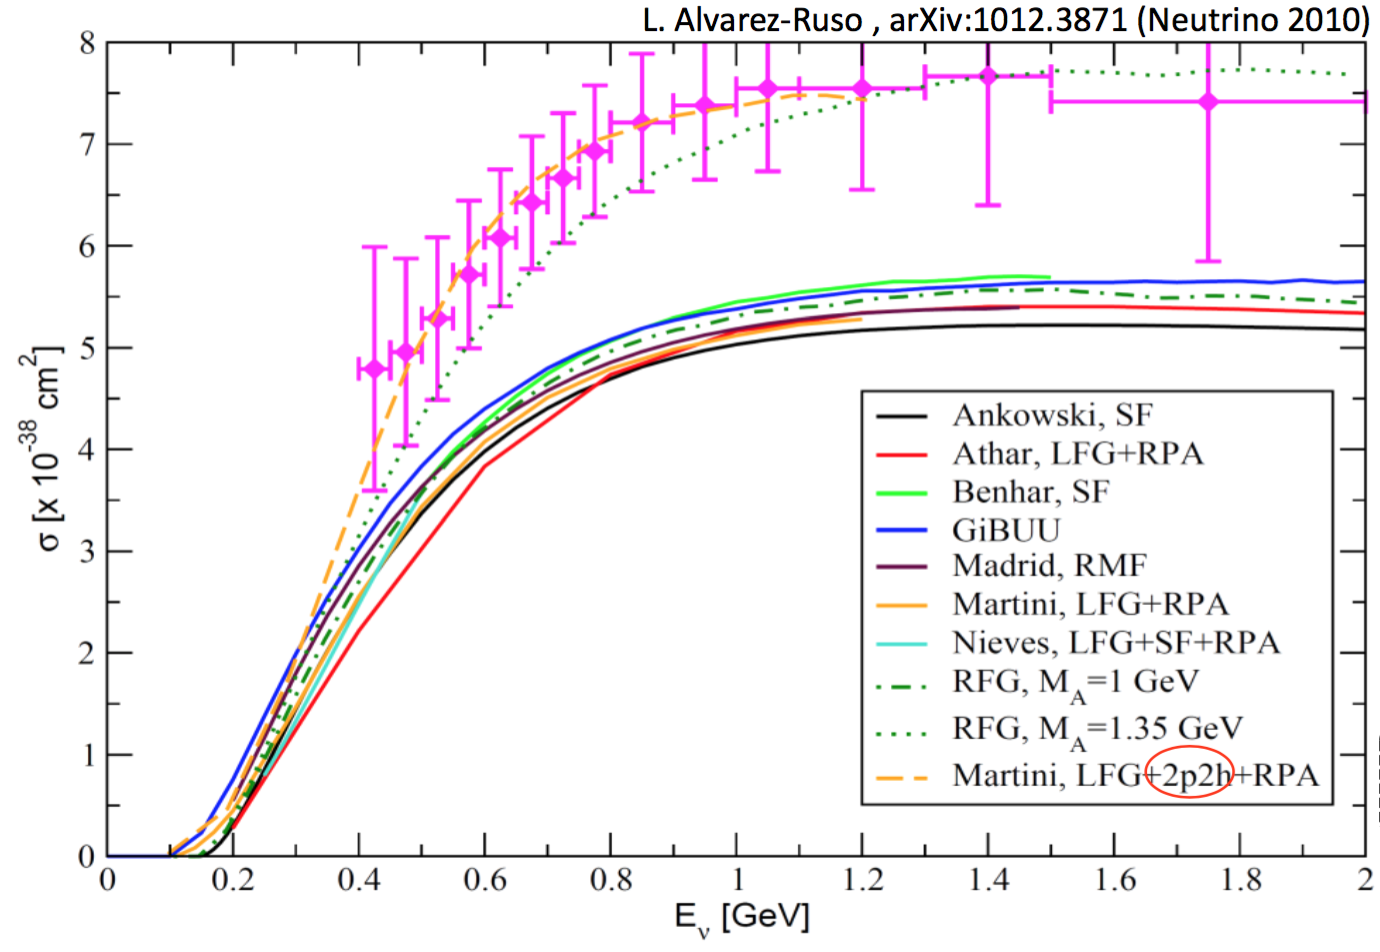
\includegraphics[width=0.90\textwidth]{./images/nuint/ccqe/qe_puzzle}\\
      \end{center}
    \end{column}
    \begin{column}{0.58\textwidth}
      {\scriptsize
       \begin{center}
         {\color{cadmiumred} T2K 1-ring e-like candidates in $\nu$ mode}:\\
         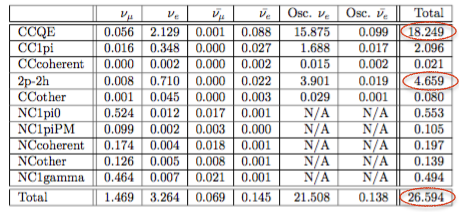
\includegraphics[width=0.90\textwidth]{./images/nuint/other/T2KFHC1ReRun1to7_annotated}\\
       \end{center}
       {\bf On single nucleons}, this process is {\bf theoretically understood and
       well constrained} by experimental information from
       \begin{itemize}
          \item electron scattering, neutron $\beta$ decay, and
          \item $\nu$ experiments on Hydrogen/Deuterium.
       \end{itemize}
       {\bf Unable to describe nuclear QE-like data} with models
       based on interactions on single nucleons alone.\\
     }
    \end{column}
  \end{columns}

\end{frame}

%
%
%
\begin{frame}{The QE puzzle: Two-nucleon interactions}

{\small
 The observed dicrepancy revealed the {\color{cadmiumred}importance of two-nucleon interactions}.
 This was further stressed by ab-initio calculations of nuclear response functions.
}

  \begin{columns}
    \begin{column}{0.70\textwidth}
      \begin{center}
        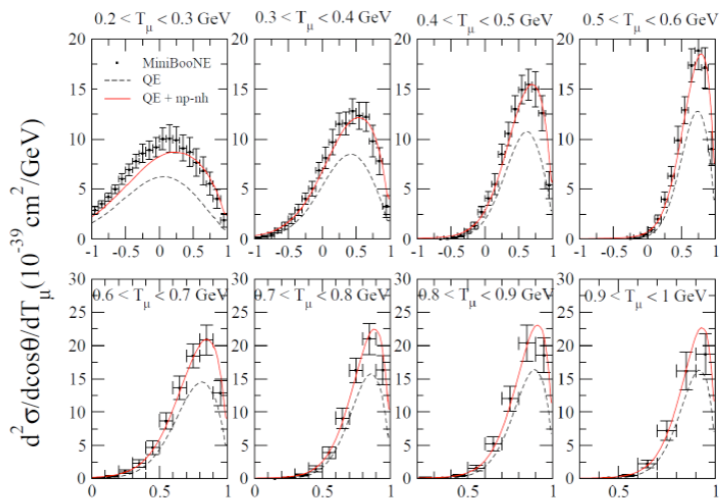
\includegraphics[width=0.98\textwidth]{./images/nuint/ccqe/martini_2p2h.png}\\
        {\scriptsize [Martini et al. PRC 84 055502 (2011)]; MiniBooNE data shown}
      \end{center}
    \end{column}
    \begin{column}{0.30\textwidth}
     \begin{center}
        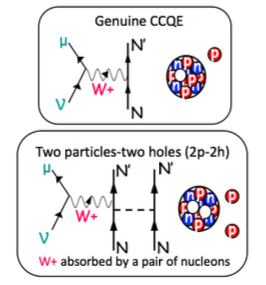
\includegraphics[width=0.95\textwidth]{./images/nuint/feyn/2p2h_diagrams_2.png}\\
        {\scriptsize
          Meson exchange between two bound nucleons\\
         (e.g through virtual $\Delta$ or contact term).
        }
     \end{center}
    \end{column}
  \end{columns}

\end{frame}

%
%
%
\begin{frame}{The QE puzzle: Two-nucleon interactions}

{\small
  Recent CC0$\pi$ measurements from T2K in agreement with
  theoretical models including 2p2h.\\}

  \begin{center}
     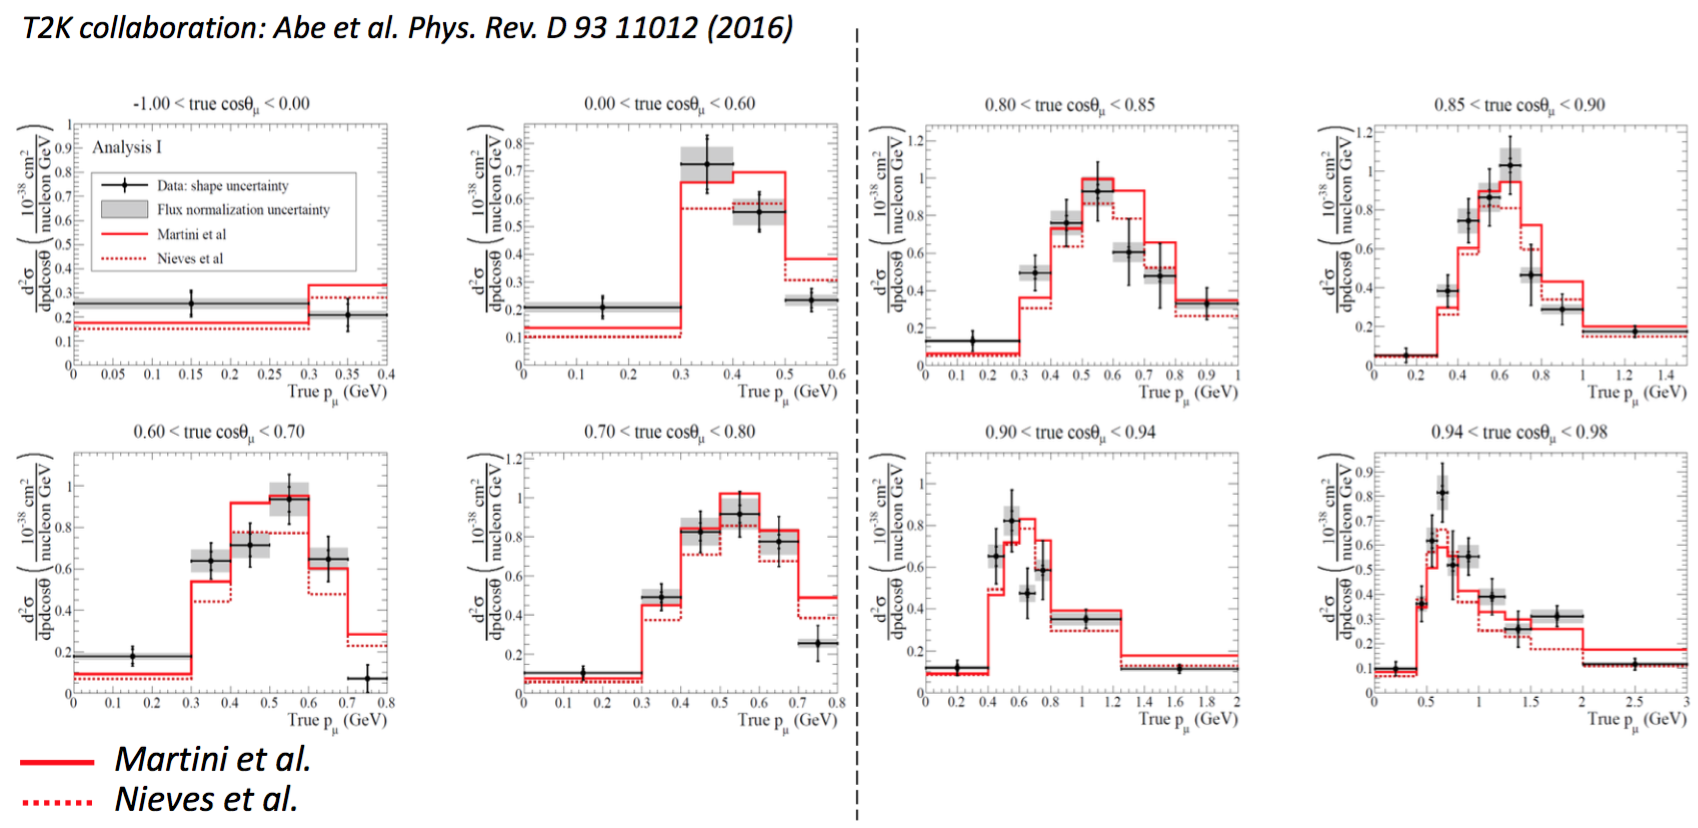
\includegraphics[width=0.95\textwidth]{./images/nuint/ccqe/t2k_cc0pi.png}\\
  \end{center}
\end{frame}

%
%
%
\begin{frame}{The QE puzzle: Identifying 2p2h events}

\begin{itemize}
{\small
  \item Characteristic events with 2 back-to-back f/s nucleons seen in ArgoNEUT.
  \item {\it "Avalanching shadows the initial reaction"} [U. Mosel]
  \item Future data from LarTPCs (or, better, gas TPCs)
        CC0$\pi$ events subdivided based on nucleon multiplicity crucial for
        disentangling FSI and 2p2h effects.
}
\end{itemize}

  \begin{columns}
    \begin{column}{0.40\textwidth}
      \begin{center}
        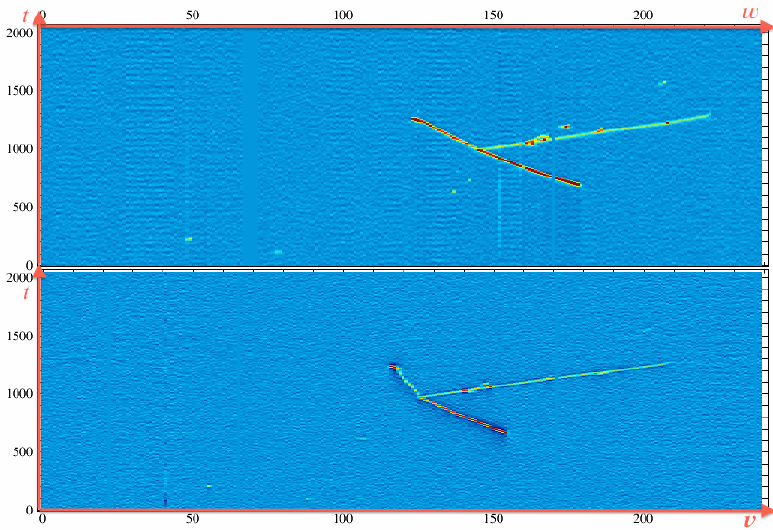
\includegraphics[width=0.99\textwidth]{./images/nuint/evdisplay/hammer_event}\\
        {\scriptsize [Phys.Rev. D90 (2014) 1, 012008]}
      \end{center}
    \end{column}
    \begin{column}{0.60\textwidth}
      \begin{center}
        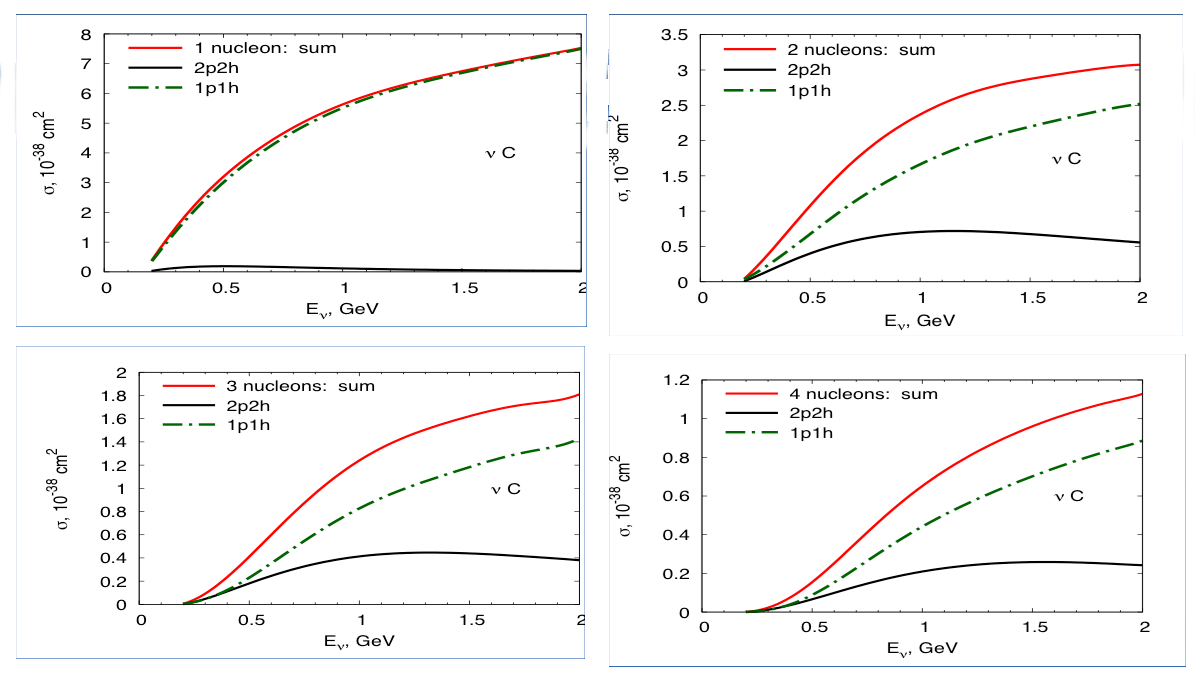
\includegraphics[width=0.99\textwidth]{./images/nuint/ccqe/npnh_gibbu}\\
        {\scriptsize Ulrich Mosel}
      \end{center}
    \end{column}
  \end{columns}

\end{frame}


%
%
%
\begin{frame}{Resolving the QE puzzle: A new approach}

  %
  % \begin{center}
  %   {\tiny [Phys.Rev. D94 (2016) no.11, 112007]}\\
  %    \includegraphics[width=0.70\textwidth]{./images/minerva_q0q3.png}\\
  % \end{center}

  \begin{columns}
    \begin{column}{0.70\textwidth}
      \begin{center}
        {\tiny [Phys.Rev. D94 (2016) no.11, 112007]}\\
         \includegraphics[width=0.98\textwidth]{./images/nuint/ccqe/minerva_q0q3.png}\\
      \end{center}
    \end{column}
    \begin{column}{0.30\textwidth}
      {\scriptsize
        New approach by MINERvA:\\
        {\bf Inclusive $\nu_{\mu}$ CC data
        in $(q_0, |\vec{q_3}|)$ space}.\\
        Exploiting the different kinematical dependency
        of each component to disentangle 2p2h.\\
      }
    \end{column}
  \end{columns}

  % NOVA
  \begin{columns}
    \begin{column}{0.30\textwidth}
      {\scriptsize
        Similar approach by NOvA.\\
        {\tiny [Phys.Rev. D93 (2016) no.7, 071101]}\\
        }
    \end{column}
    \begin{column}{0.70\textwidth}
     \begin{center}
        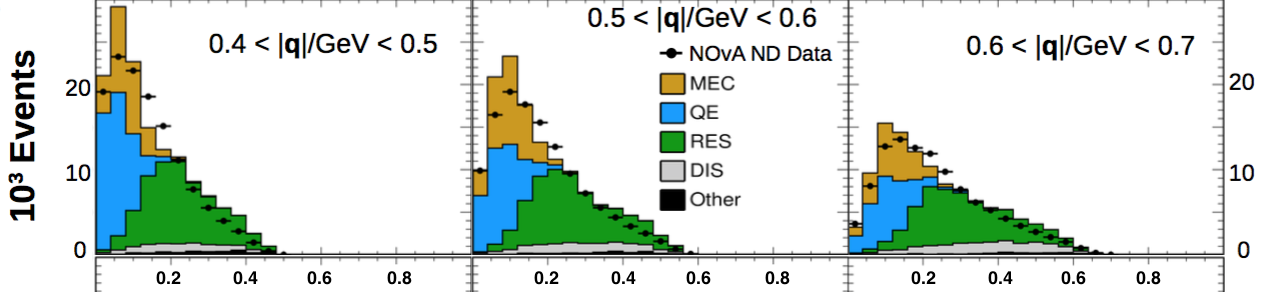
\includegraphics[width=0.95\textwidth]{./images/nuint/ccqe/nova_q0q3_few_bins.png}\\
     \end{center}
    \end{column}
  \end{columns}

\end{frame}


%
%
%
\begin{frame}{Resolving the QE puzzle: Why is this important?}

{\small
  Effective models (e.g. inflated axial mass)
  give reasonably good phenomenological description.
  Why is it important to understand the micro-physics?\\
}

\vspace{0.1cm}

  \begin{columns}[T]
    \begin{column}{0.50\textwidth}
    {\scriptsize
      {\bf Energy reconstruction}\\
      1p1h/2p2h mixture drives the mapping between
      true and reconstructed energy!\\
      \begin{center}
        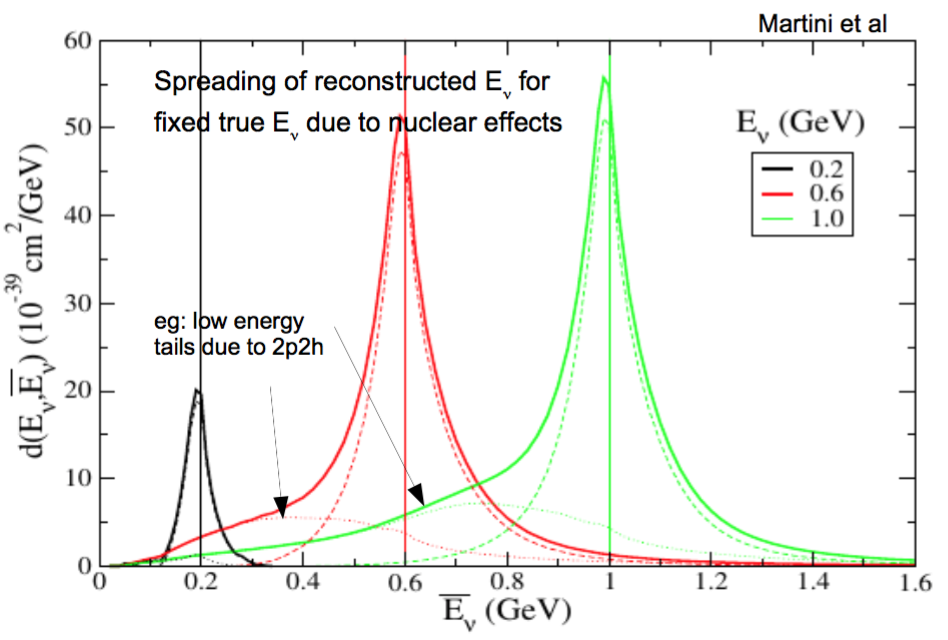
\includegraphics[width=0.99\textwidth]{./images/nuint/ccqe/ErecoQE_martini}
      \end{center}
      \noindent\rule{2cm}{0.4pt}\\
        (*) $A_{CP} \propto \frac{sin2\theta_{12}}{sin\theta_{13}} sin\delta_{CP}$
    }
    \end{column}
    \begin{column}{0.50\textwidth}
    {\scriptsize
     {\bf CP sensitivity}\\
     Large measured $\theta_{13}$, yields
     large $\nu_{e}$ and $\bar{\nu}_{e}$ appearance rate,
     but smaller CP asymmetry (*).\\
     Appearance {\bf signal systematics} important.\\
     Models predict differ in $\nu$/$\bar{\nu}$ 2p2h.\\
     \begin{center}
        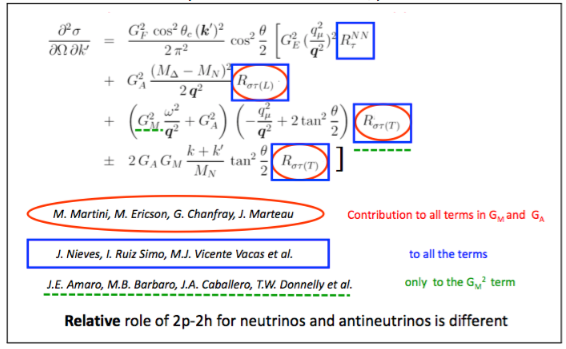
\includegraphics[width=0.99\textwidth]{./images/nuint/ccqe/martini_3models_nunubar.png}\\
        {\tiny [Martini, INT 2013, Seattle]}
     \end{center}
    }
    \end{column}
  \end{columns}

\end{frame}


%
% NCEL
%





%
% What you should know
%

\begin{frame}{What you should know}

\end{frame}


%
% What to read
%

\begin{frame}{What to read}

\begin{itemize}
{\scriptsize

\item
{\it H. Gallagher, G.Garvey and G.Zeller},
Neutrino-Nucleus Interactions,
Annu.Rev.Nucl.Part.Sci. 2011, 61:355-78

\item
{\it G.Garvey, D.Harris, H.Tanaka, R.Tayloe and G.Zeller},
Recent Advances and Open Questions in Neutrino-Induced Quasi-Elastic Scattering and Single Photon Production,
arXiv:1412.4294

\vspace{0.1cm}
\item
{\it A.Bodek, E.Christy and B.Coopersmith},
Effective Spectral Functions for Quasi-Elastic Scattering on Nuclei,
arXiv:1405.0583

\vspace{0.1cm}
\item
A. Aguilar-Arevalo et al. [MiniBooNE Collaboration],
Phys. Rev. D 81, 092005 (2010); arXiv:1002.2680 [hep-ex]

\vspace{0.1cm}
\item
A. A. Aguilar-Arevalo et al. [MiniBooNE Collaboration],
Phys. Rev. D 88 (2013) 3, 032001; arXiv:1301.7067 [hep-ex]

}
\end{itemize}

\end{frame}
